\chapter{Global continuation theory}\label{chap3} %% chap 3

\section{Introduction}\pageoriginale\label{chap3-sec3.1}%sec 3.1

 In this section we will discuss some preliminary aspects which are
  useful  in the study of {\bf global continuation results}. We will start
  with some definitions regarding the function $G$ from $\mathbb{R}^M$
  into $\mathbb{R}^N$.    
  The Jacobian of $G(x)$ is:
  $$
  G' (x) = \frac{\partial G}{\partial x} (x) = ( \frac{g_i}{x_j} (x_1, 
  \ldots , x_M))_{\substack{1 \leq j \leq M\\ 1 \leq i \leq N}}, 
  $$
  where $x=(x_1, \ldots x_M)T$ and $G=(g_1, \ldots g_N)^T \cdot G'(x)$ is
  an $N \times M$ matrix and its rank must be less than or equal ti
  min $(N, M)$.

\begin{defins*} 
\begin{enumerate}
\renewcommand{\labelenumi}{(\theenumi)}
\item Let $G$ be continuously differentiable. Let 
$$
C =  \{ x \in  \mathbb{R}^M : \text{ Rank } G' (x) < \min (N,M)\}.
$$ 

The points in $C$ are called critical points of $G$. 

\item The regular points are the points in the complement  of $C$,
  denoted by $\mathbb{R}^M \, \backslash \, C$. 

\medskip
\noindent\textbf{Note:}
The domain $\mathbb{R}^M$ can always be replace by the
closure of an open set in $\mathbb{R}^M$. 

\item The\pageoriginale image  of the set $C$ under $G$, i.e. $G(C)$
  which is a subset 
  of $\mathbb{R}^N$ is the set of critical values of $G$. 

\item The complement of $G(C)$ in $\mathbb{R}^N$ is the set of regular
  values of $G$. i.e. $\mathbb{R}^N \, \backslash \, G(C)$. 
\end{enumerate}
\end{defins*}

Now we will state and prove {\em Sard's Theorem} (See \cite{key26}). 

\section{Sard's Theorem}\label{chap3-sec3.2}%sec 3.2
  
\textit{Let $G \in C^1 ( \mathbb{R}^M) \cap
    C^{M-N+1}(\mathbb{R}^M)$. Then $G(C)$ has $\mathbb{R}^N $ -
    measure zero}. 

\begin{proof}
We will prove the result for $M=N$. The case $M < N$ is trivial. In
this case there exist a nontrivial null vector of $G'$. This is
precisely the idea we are going  to use in the case $M=N$. For $M >N$
see \cite{key1}. 
  
  So assume $M=N$. Let  $Q_0$ be an arbitrary cube in $\mathbb{R}^N$
  of side $L$. (Therefore vol $(Q_0)= L^N$). We will show that volume
  $(G(C \cap Q_0))$ is zero which implies that the measure of $G(C)$
  is zero, since $L$ is arbitrary. 

 
  With $\ell = \frac{L}{n}$, let $\{ q_j\}$ be the set cubes of side
  $\ell$, for $j=1,2 , \ldots n^N$, which form a partition of
  $Q_0$. i.e.  
  $$
  Q_0=\bigcup_{j=1}^{n^N} q_j. 
  $$
  
  Assume that each $q_j$ contains at least one critical point, say
  $x^j$. Let $x \in q_j$, then  
\begin{align*}
G(x) & = G(x^j + (x-x^j))\\
& = G(x^j) + G'(x^j)(x-x^j) + o (\ell ),
\end{align*}  
where $\dfrac{o(\ell)}{\ell} \to 0$ as $\ell \to 0$. 

Using\pageoriginale the fact that, rank $G' (x^j) \le N-1$, we will
show that for  
sufficiently small $\ell$, $z^j(x) = G'(x^j)(x-x^j) $ lies in $N-1$
dimensional subspace of $\mathbb{R}^N$ as $x$ varies. To see this, let
$\xi^j$ be a unit null vector of $G'(x^j)$. Put 
$$
y^j(x) = x-x^j = [y^j - < y^j, \xi^j > \xi^j] + < y^j, \xi^j > 
\xi^j. 
$$

Note that the vector $y^j - < y^j$, $\xi^j > \xi^j$ has no component in
the $\xi^j$ direction and hence it lies in an $N-1$ dimensional
subspace of $\mathbb{R}^N$. As $x$ varies over $q_j$, all these
vectors $\{ z^j(x) \}$ lie in the same $N-1$ dimensional
subspace. Since $G'(x^j)$ is independent of $x$, the measure of the
set  
$$
\{ G' (x^j)y^j(x) : x \in q_j \} 
$$
is less than or equal to $(K \ell)^{N-1}$, where $K$ is a constant
(maximum elongation constant for $G$ on $Q_0$). Hence the volume of
$\{ G' (x^j)y^j (x) + o (\ell): x \in q_j \}$ is less than or equal to
$(K \ell)^{N-1} \times  o(\ell)$. Thus  
\begin{align*}
{\rm Vol} \{ G (C \cap Q_0) \} & \leq n^N (C\ell )^{N-1} o(\ell ) \\ 
& = (C^{N-1} L^{N}) \frac{o(\ell )}{\ell} \rightarrow 0 \text{ as }
\ell \rightarrow 0. 
 \end{align*} 

This proves Sard's theorem for the case $M \leq N$.
\end{proof}

\section{Examples}\label{chap3-sec3.3}

\begin{enumerate}
\renewcommand{\labelenumi}{(\theenumi)}
\item Consider the example from population dynamics:
$$
G(u, \lambda) = u^2 - \lambda_1 u - \lambda_2 .
$$

Take 
\begin{equation*}
x\equiv
\begin{bmatrix}
x_1 \\ x_2 \\ x_3   
\end{bmatrix}
=
\begin{bmatrix}
u \\ \lambda_2 \\ \lambda_3  
\end{bmatrix}.
\end{equation*}

Then\pageoriginale $G(u, \lambda)$ and its derivative can be written as 
\begin{align*}
G(x) & = x^2_1 -x_2 x_1 -x_3, \\
G'(x) &=  [2x_1 - x_2, -x_1, -1].
\end{align*}

Rank $(G'(x)) = 1$, which is the maximum rank. Therefore there are no
critical points for this problem. 

\item Define $G: \mathbb{R}^2 \rightarrow \mathbb{R}$ by:
$$
G(x) = x^2_1 -x_2 x_1 -k \text{ \ where $k$ is a constant.}
$$
 \end{enumerate}  

Then
$$
G'(x) = [2x_1 -x_2, -x_1].
$$
and it has the maximum rank 1, except at $x = (0,0)$ where $G'(x)$
has rank zero. This is a critical point and it is the only critical
point. The critical value is $G(0) = -k$. 
 
Observe that the solution curves of $G(u) = 0$ are two disjoint
curves for $k \neq 0$. For $k=0$ they are two lines which intersect
at the origin, which is a bifurcation point. See
Fig.~\ref{chap3-fig3.1}.  

\begin{figure}[H]
\centering
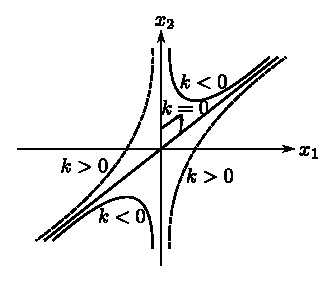
\includegraphics{vol79-fig/fig79-19.eps}
\smallskip
\caption{}\label{chap3-fig3.1}
\end{figure}


\section{Solution sets for Regular
  Values}\pageoriginale\label{chap3-sec3.4}%sec 3.4 
 
We study now the solutions of $G(x) = p$, Where $p$ is a regular
value. 
 
\section{Lemma (Finite Set of Solutions)}\label{chap3-sec3.5}%sec 3.5

\textit{Let $G : \mathbb{R}^N \rightarrow \mathbb{R}^N$ with
$G \in C^1 (\bar\Omega)$, for some bounded open set $\Omega
\subset \mathbb{R}^N$. Let $p \in \mathbb{R}^N$ be a regular
  value of $G$ such that}: 
$$
G(x) \neq p  \text{ \ for \ } x \in \partial\Omega.
$$

\textit{Then the set $G^{-1}(p) \cap \bar{\Omega}$ is finite, where}:
$$
G^{-1}(p)  = \{ x \in \mathbb{R}^N : G(x) = p \}.
$$

\begin{proof}
We give a proof by contradiction. Let $\{ x_j \}^\infty_{j = 1} \in
G^{-1} (p) \cap \bar{\Omega}$ and assume all $x_j$'s are
distinct. Then some subsequence of $\{ x_j \}$ converges to some $x^*
\in \bar{\Omega}$. By the continuity of $G$, we have: 
$$
G(x^*) = p.
$$

This implies $x^* \notin \partial \Omega$. However by the implicit
function theorem, there is one and only one solution $x = x(p)$ of
$G(x) = p$ in some open neighbourhood of $x(p)$. This is a
contradiction, since every neighbourhood of $x^*$ contains infinitely
may $x_j$'s. This complete the proof. 
\end{proof}

Next, we will consider the case $G : \mathbb{R}^{N+1} \rightarrow
\mathbb{R}^N$ and study the solution set $G^{-1}(p)$, if $p$ is a
regular value. 

\section{Lemma (Global Solution Paths)}\label{chap3-sec3.6}%sec 3.6

\textit{Let $G : \mathbb{R}^{N+1} \rightarrow \mathbb{R}^N, $
and $G \in C^2 (\mathbb{R}^{N+1})$. Let $p$ be a
  regular value\pageoriginale for $G$. Then $G^{-1} (p)$ is a $C^1$,
one dimensional manifold. That is each of its connected
components is diffeomorphic to a circle or infinite interval. In more
  detail, each component of $G^{-1}(p)$ can be represented by
  a differentiable function $X(s)$, $s \in \mathbb{R}$ and it
  satisfies one of the following}: 
\begin{equation*}
\begin{array}{r@{\;\;}l}
\text{(a)} & ||X(s)||\rightarrow \infty \text{ \ as\ } |s|
\rightarrow \infty.\\  
\text{(b)} & {X(s)} \text{ is a simple closed curve and $X(s)$
is periodic.}\\ 
\text{(c)} & G^{-1} (p) = \phi.
\end{array}\tag{3.6}\label{chap3-sec3.6-eq3.6}
\end{equation*}

\begin{proof}
Assume that $G^{-1}(p) \neq \phi$, or else we are done. Let $x^0$ be
such that:  
$$
G(x^0) - p = 0.
$$

Consider the equation:
$$
G(x) - p = 0.
$$

Since $p$ is regular value, the Jacobin of $G(x)-p$ at $x^0$
viz. $G'(x^0)$, must have the maximum rank $N$. Therefore, it has a
minor of order $N$, which is nonsingular. Assume that $\dfrac{\partial
  G}{\partial(x_1, , ,x_N)} (x^0)$ is nonsingular. Let $(x_i, ..x_N) =
u$ and $x_{N+1} = \lambda$. Thus we have: 
$$
F(u^0 , \lambda^0) \equiv G(u^0 , \lambda^0) - p = 0 ,
$$
and  
$$
F_u(u^0 , \lambda^0) = G_u(u^0 , \lambda^0) 
$$
is nonsingular. Hence by the implicit function theorem there exists a
unique solution $u = u(\lambda)$, for all $\lambda$ such that
$|\lambda - \lambda^0| < p_1(u^0,
\lambda^0)$. i.e. there\pageoriginale exits a solution are: 
$$
\gamma^1 = \{ x_1 (x_{N+1}), \ldots, x_N(x_{N+1}), x_{N+1} \}, 
$$
with $X_{N+1}$ in some iterval $|x_{N+1} -x^0_{N+1}| <
\rho_1(x^0)$. Extend this arc over a maximal interval (the interval
beyond which we cannot extend the solution), say, $x^L_{N+1} < x_{N+1}
< x^R_{N+1}$. 
\begin{figure}[H]
\centering
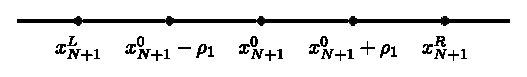
\includegraphics{vol79-fig/nonum.eps}
\end{figure}

At the points, the Jacobian $\dfrac{\partial G}{\partial (x_1, ..x_N)}
(x^0)$ will be singular, otherwise we can again apply implicit
function theorem to obtain the solution in a larger interval which
will contradict the maximality of the interval. Now consider the point
$x^R = (x_1(x^R_{N+1}),\ldots (x_N(x^R_{N+1}), x^R_{N+1})$. By the
continuity of $G$ we have: 
$$
G(x^R) =p.
$$

Again since $p$ is a regular value, there exists a minor of rank $N$,
which is nonsingular. Assume that this is obtained from the matrix
$G_x$ by removing the $j^{\text{th}}$ column of the matrix. As before, there
exists an are $\gamma^2$, say, 
$$
\gamma^2 = \{ x_1 (x_j),\ldots x_{j-1}(x_j), x_j, x_{j+1} (x_j),\ldots
x_{N+1} (x_j) \},  
$$
over a maximal interval. We can continue this procedure
indefinitely. This family $(\gamma^i)$ will overlap because the
implicit function theorem gives a unique curve. Thus $\{ \gamma^i \}$
form a $C^1$ curve. This curve can be globally parametrized. Suppose
it is given by: 
$$
 \Gamma = \{ X(s); X(s_a) = x^0, s_a \leq s \leq s_b \}   
 $$\pageoriginale
and 
$$
G(X(s)) = p.
$$

If $X(s)$ is not bounded, then the first part of the theorem
follows. So assume that $X(s)$ is bounded. Then choose a sequence $\{
s_j \} \rightarrow \infty$ such that $\{ X(s_j) \} \rightarrow
x^*$. By the continuity of $G$ we get: 
$$
G(x^*) = p.
$$

If the curve is not closed, $x^*$ will be a limit point and also a
solution of $G(x)-p = 0$. Since $p$ is a regular value, we can apply
the implicit function theorem to conclude that the curve has to be
closed. This closed curve is simple, because of the uniqueness of the
solution path. Hence in the case when $X(s)$ is bounded, we have a
simple closed periodic solution which proves part $(b)$ of the
theorem. 
\end{proof}

\begin{remark*}
The main idea in the proof is the change of parameter from one
component $\gamma^j$ to another. This can be used as a practical
procedure for carrying out global continuation; see \cite{key27}. 
\end{remark*}


\section{Degree Theory}\label{chap3-sec3.7}%sec 3.7

In this section we will assign an integer, called the `\textbf{degree}' to a
continuous function $F$, defined on an open subset $\Omega$, of
$\mathbb{R}^N$ and a point $p \in \mathbb{R}^N$. This is an
important tool in proving fixed point theorems and existence results
for nonlinear problems. The degree of a continuous function $F$ over
a domain at a point $p$ has the important property that if it is non -
zero, then there exists a solution of $F(x) = p$ in\pageoriginale the given
domain. Another important property is that it depends on the values of
the function only on the boundary and not in the interior. 

\section{Definition}\label{chap3-sec3.8}%3.8

Let $F : \mathbb{R}^N \rightarrow \mathbb{R}^N$ and $p  \in
\mathbb{R}^N$ satisfy: 
\begin{enumerate}[(i)]
\item $F \in C^1 (\bar{\Omega})$, where $\Omega$ is an open
  bounded subset of $\mathbb{R}^N$, 

\item $p \not\in F (\partial \Omega)$,

\item $p$ is a regular value of $F$ on $\Omega$. 
\end{enumerate}

Then the degree of $F$ on $\Omega$ for $p$ is defined as:
\begin{equation*}
\deg (F, \Omega , p) = \sum_{x \in [F^{-1} (p) \cap \bar{\Omega}]}
{\rm Sgn} [\det F'(x)].\tag{3.8}\label{chap3-sec3.8-eq3.8} 
\end{equation*}

\begin{note*}
The degree is well defined, since by lemma \ref{chap3-sec3.5},
$[F^{-1} (p) \cap \bar{\Omega}]$ is a finite set and hence the right
hand side is a finite sum. 
\end{note*}

\begin{example*}
Consider $f: \mathbb{R} \rightarrow \mathbb{R}$ such that $f'(x)$ is
continuous on [$a$, $b$] and $f(a) \neq p$, $f (b) \neq p$ and $f(x) = p$
has only simple roots on [$a$, $b$]. Then  
$$
\deg (f,(a,b),p) = \sum^k_{j=1} \frac{f'(x_j)}{|f' (x_j)|},
$$
where $\{ x_j \}^k_{ j=1}$ are the consecutive roots of $f(x) - p = 0$
contained in [$a$, $b$]. In this particular case, if $f'(x_j) > 0$, then
$f'(x_{j +1}) < 0$ and vice versa. Therefore
$\dfrac{f'(x_j)}{|f'(x_j)|} = + 1$ and $-1$ alternatively. Hence  
$$
\deg (f,(a,b),p) \in \{ 1,0, -1 \}.
$$

Now if $p$ does not lie between $f(a)$ and $f(b)$, then there are
either no\pageoriginale roots or an even number of roots for the
equation $f(x) = p$ 
in ($a$, $b$). Hence the degree is zero. In the other case, there will
be an odd number of roots, say $(2k+1)$, $k \geq 0$. Thus in the
summation in \eqref{chap3-sec3.8-eq3.8}, 
the first $(2k)$ terms cancel out and the last
term is $+1$ or $-1$, depending on $f(b) > p$ or $f(b) < p$. Hence we
can write: 
$$
\deg  (f,(a,b),p) = \frac{1}{2} \left[ \frac{f(b)-p}{|f(b)-p|} - \frac{f(a)
    -p}{|f(a)-p|}\right]. 
$$

Note that in this case the degree depends only on the values of $f$ at
the boundary points $a$ and $b$. This is true in the general case
also.  

Next we will relax condition (iii) of definition \ref{chap3-sec3.8}.
\end{example*}

\section{Definition}\label{chap3-sec3.9}%sec 3.9

Let $F$  satisfy (i) and (ii) of \eqref{chap3-sec3.8}. Then, 
\begin{equation*}
\deg (F, \Omega , p) \equiv \deg (F, \Omega, q),
\tag{3.9a}\label{chap3-sec3.9-eq3.9a} 
\end{equation*}
where $q$ satisfies:  
\begin{equation*}
\begin{array}{r@{\;\;}l}
\text{(i)} & q \text{ is a regular value of } F,\\ 
\text{(ii)} & || q-p || < \gamma \equiv \text{ dist }(F(\partial
\Omega ),p) \equiv \inf_{x \in \partial \Omega} || F(x) - p ||. 
\end{array}\tag{3.9b}\label{chap3-sec3.9-eq3.9b}
\end{equation*}

By Sard's theorem, the set of all regular values of $F$ are dense in
$\mathbb{R}^N$. Hence we can find regular values satisfying
(\ref{chap3-sec3.9-eq3.9b}(ii)). 
Also if $q_1$, $q_2$ are two regular values satisfying
(\ref{chap3-sec3.9-eq3.9b}(ii)), then they belong to the same
connected component of 
$\mathbb{R}^N \, \backslash \,  F(\partial \Omega)$ and hence (for a
proof which is too lengthy to include here see \cite{key29}): 
$$
\deg (F, \Omega, q_1) = \deg (F, \Omega, q_2). 
$$

Therefore the above degree is well defined. We can also relax
condition (i)\pageoriginale of definition \ref{chap3-sec3.8} and
define the degree for $F \in C(\bar{\Omega})$.  


\section{Definition}\label{chap3-sec3.10}%defini 3.10
Assume $F$ satisfies:
\begin{enumerate}[(i)]
\item $ F \in C (\bar{\Omega})$.

\item $p \notin F (\partial \Omega)$.

Then 
\begin{equation*}
\deg (F, \Omega , p ) \equiv \deg (\tilde{F}, \Omega , p)
\tag{3.10}\label{chap3-sec3.10-eq3.10} 
\end{equation*}
where $\tilde{F}$ satisfies, using $y$ of (\ref{chap3-sec3.9-eq3.9b}(ii)):

\item $\tilde{F} \in C^1 (\bar{\Omega})$,

\item $|| F - \tilde{F}||_\infty < \dfrac{\gamma}{2}$. 
\end{enumerate}

Since $F$ is continuous, we can approximate $F$ as closely as desired,
by differentiable function $\bar{F}$. (Take polynomials, for
example). Conditions (ii) and (iv) imply that $p \not\varepsilon
\tilde{F} (\partial \Omega)$. Thus deg $(\tilde{F}, \Omega, p)$ is
well defined by definition \ref{chap3-sec3.9}. If $\hat{F}$ is another smooth
function, satisfying condition (iv), then by considering the
homotopy 
$$
G(x,t) = t \tilde{F}(x) + (1 - t) \hat{F}(x) 
$$ 
and using the homotopy invariance property of the degree in definition 
\ref{chap3-sec3.8} (which we prove next), it follows that 
$$
\deg (\tilde{F}, \Omega, p) = \deg (\hat{F}, \Omega, p). 
$$

Thus definition \ref{chap3-sec3.10} is independent of the choice of
$\tilde{F}$. Thus the degree is well defined even for a function $F
\in C(\bar{\Omega})$.  


\section{Theorem (Homotopy Invariance of the
  Degree)}\label{chap3-sec3.11}\pageoriginale%sec 3.11 

\textit{Let $G : \mathbb{R}^{N+1} \rightarrow \mathbb{R}^N$, $\Omega$
bounded open set in $\mathbb{R}^N$ and $p \in
\mathbb{R}^N$ satisfy}: 
\begin{equation*}
\begin{array}{r@{\;\;}p{6.5cm}}
\text{(a)} &  $G \in C^2 (\bar{\Omega} \times 
   [0,1])$, \\
\text{(b)} & $G(u, \lambda) \neq p$  \ on\  $\partial \Omega
\times   [0,1]$,\\ 
\text{(c)} & $G(u, 0) \equiv F_0 (u)$, $G(u,1) \equiv F_1(u)$,\\
\text{(d)} & $p$  \ is a regular value for  $G$ on\newline
  $\bar{\Omega} \times  [0,1]$  \ and for \ $F_0$
 \ and\  $F_1$ on $\bar{\Omega}$. 
\end{array}\tag{3.11}\label{chap3-sec3.11-eq3.11}
\end{equation*}

\textit{Then $\deg (G(.,\lambda), \Omega, p)$ is independent
  of $\lambda \in [0,1]$. In particular,} 
$$
\deg (F_0, \Omega , p) = \deg (F_1, \Omega , p). 
$$


\begin{proof}
The proof uses lemma \ref{chap3-sec3.5}. We will prove 
$$
\deg (F_0,
\Omega , p) = \deg (F_1, \Omega , p).
$$

The case for any $\lambda \in
(0,1)$ is included. Since $p$ is a regular value, we have:  
$$
\{ F^{-1}_0 (p) \cap \bar{\Omega} \} = \{u^0_i \},
$$
and 
$$
\{ F^{-1}_0 (p) \cap \bar{\Omega} \} = \{ u^1_j \}, 
$$
where $\{ u^0_i \}$ and $\{ u^1_j \}$ are finite sets by lemma
\ref{chap3-sec3.5}. Again, since $p$ is a regular value, $\{ G^{-1}(p)
\cap (\bar{\Omega} \times [0,1]) \}$ is a finite collection of arcs,
denoted by $\{ \Gamma_i (s)\}$. Let us parametrize any $\Gamma(s)$ as
$(u(s), \lambda(s))$, where $s$ denotes the arc length. On $\Gamma(s)$
we have: 
$$ 
G(s) \equiv G(u(s), \lambda(s)) = p. 
$$

Differentiating\pageoriginale with respect to $s$, we get :
$$
G_u(s) \cdot \dot{u}(s) +  G_\lambda (s) \dot{\lambda} (s) = 0. 
$$

Since $s$ is the arc length, we have:
$$
\dot{u}^T (s) \dot{u}(s) + \dot{\lambda} (s) \dot{\lambda} (s) = 1.
$$

These two equations together can be written as:
\begin{equation*}
A(s) \;\; \binom{\dot{u}(s)}{\dot{\lambda} (S)} = \binom{0}{1} ,
\tag{3.12a}\label{chap3-sec3.11-eq3.12a} 
\end{equation*}
where
\begin{equation*}
A(s) =
\begin{bmatrix}
G_u(s) & G_\lambda (s) \\
\dot{u}^T(s) & \dot{\lambda} (s) .
\end{bmatrix}
\end{equation*}

We shall show that $A(s)$ is nonsingular on $\Gamma(s)$. First observe
that at each point on $\Gamma(s)$, there is a unique tangent to the
path. The matrix $[G_u(s), G_\lambda(s)]$ has rank $N$, since $p$ is a
regular value. Thus the null space of this matrix is one
dimensional. Let is be spanned by the vector $\{ \xi, n \}$. Since
$(\dot{u},  \dot{\lambda})$ is also a null vector, we have: 
$$
(\dot{u}(s), \dot{\lambda}(s)) = c_1 (\xi, \eta), \text{ \ for some\ }
c_1 \neq 0. 
$$

Now if $A(s)$ is singular, then it must have a nontrivial null vector
of the form $c_2(\xi, \eta)$ for $c_2 \neq 0$. Since 
$$
c_2 A(s) (\frac{\xi}{\eta}) = 0,
$$
the last equation gives: 
$$
c_1c_2 (| \underset{\sim}{\xi} |^2 + \eta^2) = 0.
$$

This\pageoriginale implies that $c_1 c_2 = 0$, a contradiction. Hence
$A(s)$ is nonsingular.  

Now apply Cramer's rule to solve the above system for $\lambda (s)$ to
get: 
\begin{equation*}
\dot{\lambda} (s) = \frac{\det G_u(s)}{det A(s)}
\tag{3.12b}\label{chap3-sec3.11-eq3.12b} 
\end{equation*}

Note that on $\Gamma(s)$,  det $A(s) \neq 0$.  The above result shows
that $\dot{\lambda} (s)$ and det $G_u (s)$ change sign simultaneously. 

We have by \eqref{chap3-sec3.8-eq3.8}
\begin{align*}
\deg (F_0, \Omega , p) & = \sum_{\{ u^0_i \}} \text{ sgn} (\det F'_0
(u^0_i)), \\ 
\deg (F_0, \Omega , p) & = \sum_{\{ u^1_i \}} \text{ sgn} (\det F'_1
(u^1_i)).  
\end{align*}

Observe that the arcs $\Gamma(s)$ can be classified into four
different types : 
\begin{enumerate}[(i)]
\item arcs joining two points from $\{ u^0_i \}$

\item arcs joining two points from $\{ u'_j \}$

\item arcs joining a point $u^0_i$ to a point $ u^1_j $

\item arcs with no end points.
\end{enumerate}

We shall use the arcs of type (i), (ii) and (iii) to relate the
above two degrees. 

\begin{figure}[H]
\centering
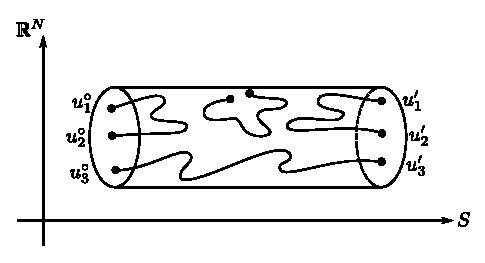
\includegraphics{vol79-fig/fig79-20.eps}
\smallskip
\caption{}
\label{chap3-fig3.2}
\end{figure}

In\pageoriginale case (i), $\dot{\lambda} (s)$ has different signs at
the end points, 
since along the $\Gamma(s)$, $\dot{\lambda}(s)$ changes sign an odd number of
times. Hence det $G_u(s)$ has different signs at the end
points. Therefore no contribution to deg $(F_0 , \Omega , p)$ results
from points. Similar result is true for case (ii). Obviously there
is no contribution to the degree from the (iv)th case. So the
only contribution comes from case (iii). Here note that $\dot{\lambda}
(s)$ and hence det $G_u (s)$ have the same sign at both the end
points, because $\dot{\lambda}(s)$ changes sign an even number of
times. This shows that:  
$$
\deg  (F_0 , \Omega , p) = \deg (F_1 , \Omega , p) 
$$
\end{proof}

The theorem is true for the other two definitions of degree
also. Indeed when these definitions have been justified, our above
proof gives the desired result with the hypothesis relaxed to
continuous mappings and without the restriction
(\ref{chap3-sec3.11-eq3.11}d).  


\section*{Some Important Properties of the Degree}
\begin{enumerate}[(1)]
\item $f$, $g : \bar{\Omega} \to \mathbb{R}^N$ be such that:
\begin{enumerate}[(i)]
\item $f(x) = g(x) $ for all $x \in \partial  \Omega$;

\item $f(x)$, $g(x) \in C (\bar{\Omega})$;

\item $f(x) \neq p$ for all $x \in \partial \Omega$;
\end{enumerate}

Then 
$$
\deg (f , \Omega , p) = \deg (g, \Omega , p). 
$$

\item If $p$, $q$ are close to each other, say,
$$
|| p-q || < \gamma = \text{dist\,} (f (\partial \Omega) ,p). 
$$

Then\pageoriginale 
$$
\deg (f_0 , \Omega , p) = \deg (f_1 , \Omega , q).  
$$

\item Let $f$, $g : \bar{\Omega} \to \mathbb{R}^N$ be continuous and $p
  \notin f(\partial \Omega) U  g(\partial  \Omega) $. Let $f$ and $g$
  satisfy  
$$
\sup_{x \in \partial  \Omega} | f(x) - g(x) | <
\frac{\gamma}{2}. 
$$

Then 
$$
\deg (f , \Omega , p) = \deg (g , \Omega , p). 
$$

\item Homotopy invariance property.

\item (Excision) If $K$ is a closed set contained in $\Omega$ and $p
  \notin f(K) U f ( \partial \Omega) $, then  
$$
\deg (f, \Omega , p) = \deg (f , \Omega  \backslash  K , p). 
$$

\item Let $p \notin f (\bar{\Omega})$, then  
$$
\deg (f, \Omega , p) = 0.
$$

\item If $\deg (f, \Omega , p) \neq 0$, then $f (x) = p$ has a
  solution in $\Omega$. (For reference, See : \cite{key26}, \cite{key29}) 
\end{enumerate}

\section*{Application 1. Fixed points and roots}

\setcounter{section}{12}
\section{Brouwer Fixed Point Theorem}\label{chap3-sec3.13}%sec 3.13

\textit{Let} $F : \mathbb{R}^N \to \mathbb{R}^N $ satisfy:
\begin{equation*}
\begin{array}{r@{\;\;}l}
\text{(a)} & F \in C (\bar{\Omega}), \Omega
 \text{ is a convex open bounded subset of } \mathbb{R}^N.\\
\text{(b)} & F (\bar{\Omega}) \subset \Omega.
\end{array}\tag{3.13}\label{chap3-sec3.13-eq3.13}
\end{equation*}

\textit{Then\pageoriginale $F(u) = u$ for some $u \in \Omega $}.

\begin{proof}
Take any point $a \in\Omega$. Define
$$
G(u , \lambda) = \lambda (u -F (u)) + (1- \lambda) (u-a) .
$$

We shall that $G$, a homotopy between $(u -F (u))$ and  $(u-a)$, does
not vanish on $\partial \Omega \times  [0,1]$. 

If $G(u , \lambda) = 0$, then we have :
$$
u = \lambda F (u) + (1 - \lambda) a
$$
By (\ref{chap3-sec3.13-eq3.13}b) we get, $F(u) \in \Omega$. Since $a
\in\Omega$, by convexity $u\in \Omega$ for $\lambda
\in [0,1]$. Therefore $G(u , \lambda) \neq 0$ on $\partial
\Omega \times [ 0,1]$. So homotopy invariance theorem implies that:  
\begin{align*}
\deg (u-F(u), \Omega , 0 ) & = \deg (u-a, \Omega ,0) \\
& = [  sgn \det \{ I \} ]_{u=a}\\
& = 1
\end{align*}
Hence $u-F(u) = 0$ has a solution in $\Omega$
\end{proof}

\begin{note*}
If $F \in C^2  (\bar{\Omega})$ the above proof is
  constructive. That is we can find arbitrarily good approximations to
  the fixed point by computation. To do this we consider:  
$$
G(u , \lambda) = \lambda (u -F (u)) + (1- \lambda) (u-a) = 0 
$$
and follow the path $\Gamma (s) $ from $(u(0), \lambda (0)) = (a,0)$,
to $(u(s_F),\lambda (s_F)) = (F(u(s_F)),1)$. If 0 is
not a regular value, we can take $\delta$ arbitrarily small and a
regular value. Then we can construct solutions for $u-F(u) =
\delta$. It\pageoriginale can be shown that 0 is a regular value for
almost all $a \in \Omega$. 
\end{note*}

Another result on global existence of a solution is given as:

\section{Theorem}\label{chap3-sec3.14}
{\em
  Let $ F \in C (\bar{\Omega})$, where $\Omega$
  is open in $\mathbb{R}^N$ and satisfy, for some}
  $x_0 \in\Omega$: 
 \begin{equation*}
< x- x_0, F(x) > > 0 \text{ for all } x \in \partial \Omega
. \tag{3.14} \label{chap3-sec3.14-eq3.14}
\end{equation*}

\textit{Then} $F(x) = 0$ \textit{for some} $x \varepsilon\Omega$.

\begin{proof}
Consider the homotopy  
$$
G(x, \lambda) = \lambda f(x) + (1 - \lambda) (x-x_0) , 0 \leq \lambda
\leq 1. 
$$

It is easy to prove that $G(x, \lambda) \neq 0$ on $\partial \Omega$
and for all $0 \leq \lambda \leq 1$. For if not, taking the inner
product with $(x-x_0)$, we get: 
$$
< x - x_0, F(x) > +  (1 - \lambda) || x-x_0 ||^2 = 0.
$$

\noindent
If $x \in \partial \Omega$ then this gives a contradiction by
\eqref{chap3-sec3.14-eq3.14}. Hence $G(x, \lambda) \neq 0$ for $ x \in
\partial \Omega$ 
and $0 \leq \lambda \leq 1$. Therefore  
$$
\deg (F , \Omega,0) = \deg (x-x_0 , \Omega,0) = 1
$$
\end{proof}


\section*{Application II. Periodic solutions of O.D.E.}

We shall use the Brouwer theorem to show the existence of periodic
solutions of systems of ordinary differential equations. 


\section{Periodic Solution Theorem}\pageoriginale\label{chap3-sec3.15}%sec 3.15

\textit{Let $f(t,y): \mathbb{R} \times \mathbb{R}^N \to \mathbb{R}^N$
  satisfy for some $T> 0$ and some convex open $\Omega \subset
  \mathbb{R}^n$}. 
\begin{equation*}
\begin{array}{r@{\;\;}>{$}p{6.5cm}<{$}}
\text{(a)} & f \in C([0,T] \times
\bar{\Omega}).\\
\text{(b)} & f(t+T,y) = f(t,y) \text{ for all } y
\in\bar{\Omega}\\ 
\text{(c)} & ||f(t,y)-f(t,x)|| \leq K ||x-y|| \text{ for all}\newline x, y
\in \bar{\Omega}, 0 \leq t \leq T, K > 0.\\
\text{(d)} & f(t,y) \text{ is directed into } \Omega  \text{ for all}\newline
 y \in \partial \Omega \text{ and } t_{\in}[0,T],
\end{array}\tag{3.15}\label{chap3-sec3.15-eq3.15}
\end{equation*}
\textit{i.e. for all $y \in \partial \Omega$, $y+ \varepsilon
  f(t,y) \in \Omega$, for all $\varepsilon> 0$ sufficiently
  small. Then the equation} 
\begin{equation*}
\frac{dy}{dt}= f(t,y) \tag{3.15e}\label{chap3-sec3.15-eq3.15e} 
\end{equation*}
\textit{has periodic solutions $y(t) $ with period $T$ and $y(t)
  \in \Omega$, for all $t$}. 

\begin{proof}
Pick any $u \in \Omega $ and solve the initial value problem : 
\begin{align*}
\frac{dy}{dt}& = f(t,y),\\
y(0) & = u.
\end{align*}

Let the unique solution in the interval $[0,T]$ be denoted by
$y(t,u)$. Then $y(t,u) \in\Omega$ for all $t > 0$. Otherwise,
let $t_1$ be the first time it crosses the boundary of $\Omega$. That
is $y(t_1, u) \in \partial \Omega$, $t_1 > 0$, $y(t,u) \in
\Omega$, for all $0 \leq t < t_1$ and,  
$$
\dot{y}(t_1,u) = f(t_1,y). 
$$


But condition (\ref{chap3-sec3.15-eq3.15}d) says that $f(t_1,y)$ is
directed into $\Omega$ 
which is not possible. Now consider $F(u) \equiv y)(T,u)$, for $u
\varepsilon\Omega$; this $F$ satisfies all the hypothesis of the
Brouwer fixed point Theorem. Hence we have: 
$$
y(T,u) = u, \text{ \ for some\ } u \varepsilon\Omega. 
$$\pageoriginale
i.e. we have a periodic solution passing through $u$.
\end{proof}

\section*{Application III. Bifurcation by degree theory}

\begin{defi*}
Let $G : \mathbb{R}^N \times \mathbb{R} \to \mathbb{R}^N$ be
$C^1$. Consider the problem:  
\begin{equation*}
G(u, \lambda) = 0. \tag{3.16}\label{chap3-sec3.15-eq3.16}
\end{equation*}

Given a smooth path (or arc) of solutions, say,
$$
\Gamma = \{ (u (\lambda) , \lambda) : \lambda_a < \lambda < \lambda_b
\}, 
$$
a point $(u^0, \lambda^0) \in \Gamma$ is said to be a
bifurcation point for \eqref{chap3-sec3.15-eq3.16} if every ball
$B_{\rho}(u^0, \lambda^0) 
\subset \mathbb{R}^{N+1}$, of radius $\rho > 0$, contains solutions of
\eqref{chap3-sec3.15-eq3.16} not on $\Gamma$. 

The following theorem shows that if the sign of det $G_u(u(\lambda),
\lambda)$ changes at some point along $\Gamma$, then it is a
bifurcation point. This is an important result in testing for
bifurcation. 
\end{defi*}

\setcounter{section}{16}
\section{Theorem (Bifurcation Test)}\label{chap3-sec3.17}%sec 3.17

\textit{Let $\Gamma$ be a smooth solution arc of
  \eqref{chap3-sec3.15-eq3.16} 
  parametrized by $\lambda$. Let det $G_u(u(\lambda),\lambda)$ change
  sign at $\lambda^0 \in(\lambda_a , \lambda_b)$. Then
  $(u(\lambda^0) \lambda^0)$ is  a bifurcation point of
  \eqref{chap3-sec3.15-eq3.16}}.  

\begin{proof}
We prove by contradiction. Assume that,
$$
(u^0, \lambda^0) = (u(\lambda^0 ) \lambda^0), 
$$
is not a bifurcation point. Hence there exists a ball of radius
$\rho$, which does\pageoriginale not contain any root of
\eqref{chap3-sec3.15-eq3.16} other on the arc 
$\Gamma$. Choose $\eta$, $\delta > 0$ small enough so that the cylinder:  
$$
C_{\eta , \delta} = \{ ( u, \lambda) : u 
\in \bar{K}_{\eta}(u^0), \lambda \in [\lambda^0 -
  \delta, \lambda^0 + \delta] \}, 
$$
where,  
$$
\bar{K}_{\eta}(u^0)= \{ u \in \mathbb{R}^N : || u - u^0 ||
\leq \eta \}. 
$$
is such that : 
\begin{enumerate}[(i)] 
\item $C_{\eta, \delta } \subset B_{\rho} (u^0 , \lambda^0)$.  

\item $G(u,\lambda) \neq 0$, for all $(u, \lambda) \in \partial 
  K_{\eta} \times [\lambda^0 - \delta, \lambda^0 + \delta] \}$. 

\item $u(\lambda^0 \pm \delta) \in K_{\eta}(u^0)$.

\item det $G_u(u(\lambda),\lambda)$ does not change sing in the
  intervals $(\lambda^0 - \delta,\lambda^0) $ and
  $(\lambda^0,\lambda^0 + \delta)$. 
\end{enumerate}

We can easily choose $\eta$ and $\delta$ so that (i) is
satisfied. Since the ball $B_{\rho}(u^0, \lambda^0)$ contains no roots
other than on the are $\Gamma$ and det $G_u (u(\lambda), \lambda)$
changes sing at $\lambda^0$ and is continuous we can shrink $\delta$
(if necessary) so that (ii), (iii) and (iv) are satisfied (see
Fig.~\ref{chap3-fig3.3}).
 
\begin{figure}[H]
\centering
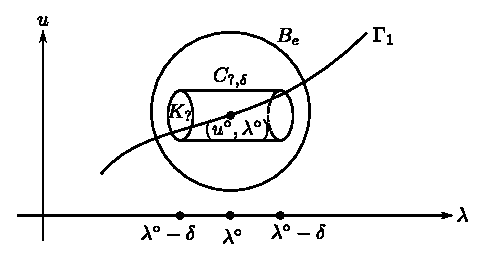
\includegraphics{vol79-fig/fig79-21.eps}
\smallskip
\caption{}
\label{chap3-fig3.3}
\end{figure}


Applying\pageoriginale the homotopy theorem to the function $G (., \lambda^0 -
\delta)$ and $G (., \lambda^0 + \delta)$, we get: 
$$
\deg (G (., \lambda^0 - \delta), K_{\eta}(u^0),0) = \deg (G (.,
\lambda^0 + \delta), K_{\eta}(u^0),0). 
$$

But 
$$
\deg (G (., \lambda^0 - \delta), K_{\eta}(u^0),0) = {\rm Sgn} \deg G_u(u ( 
\lambda^0 - \delta), \lambda^0 - \delta),  
$$ 
and 
$$
\deg (G (., \lambda^0 + \delta), K_{\eta}(u^0),0) = {\rm Sgn} \deg G_u (
u(\lambda^0 + \delta), \lambda^0 + \delta). 
$$

This is a contradiction, because det $G_u(u(\lambda),\lambda)$ has
different signs at $(u ( \lambda^0 + \delta), ( \lambda^0 - \delta)$
and $(u ( \lambda^0 + \delta), \lambda^0 + \delta)$. 
\end{proof}

\begin{note*}
 Here $\lambda^0 \in(\lambda_a,\lambda_b)$ is an interior
 point of the interval. We cannot apply this theorem if $\lambda_0$ is
 a boundary point. See Fig.~\ref{chap3-fig3.4}. 

\begin{figure}[H]
\centering
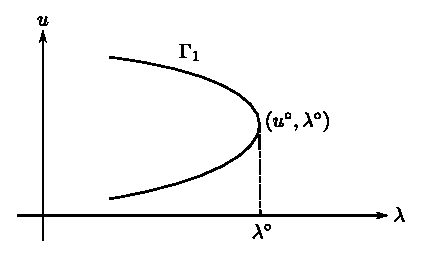
\includegraphics{vol79-fig/fig79-22.eps}
\smallskip
\caption{}
\label{chap3-fig3.4}
\end{figure}
\end{note*}

\begin{example*}
Let 
$$
G(u,\lambda) = Au - \lambda u = 0, 
$$
where\pageoriginale $A$ is an $n \times n$ symmetric matrix, $ \lambda \in
\mathbb{R} \cdot \Gamma = \{ (0, \lambda) : - \infty < \lambda < \infty \}$
is the trivial path of solutions. We have: 
\begin{align*}
\det G_u(u,\lambda ) & = \det (A - \lambda I),
& = p_n (\lambda ),
\end{align*}
where $ p_n (\lambda)$ is a polynomial in $\lambda$ of degree
$n$. Note that $ p_n (\lambda)$ changes sign at eigenvalues of odd
multiplicity. Therefore every eigenvalue of odd multiplicity
corresponds to a bifurcation point. We cannot predict anything (using
the above theorem) about the bifurcation at eigenvalues of even
multiplicity.
\end{example*}

\section{Global Homotopies and Newton's Method}\label{chap3-sec3.18}%sec 3.18

To solve 
\begin{equation*}
F(u) = 0, \tag{3.19}\label{chap3-sec3.18-eq3.19}
\end{equation*}
where $F: \mathbb{R}^N \to \mathbb{R}^N $ is a smooth function we
consider for $u^0 \in\mathbb{R}$, the homotopy: 
\begin{equation*}
G(u,t) = F(u) - e^{-\alpha t} F(u^0) \equiv
0. \tag{3.20}\label{chap3-sec3.18-eq3.20} 
\end{equation*}

Here $\alpha > 0$ and $0 \leq t < \infty$, so that when $t \to
\infty$, solution $u = u(t)$ of \eqref{chap3-sec3.18-eq3.20}, if it
exists for all $t > 
0$, must approach a solution of \eqref{chap3-sec3.18-eq3.19}. i.e. 
$$
\lim_{t \to \infty} u(t) = u^* \in F^{-1}(0).
$$

Differentiating \eqref{chap3-sec3.18-eq3.19} we get:
\begin{equation*}
F'(u) \frac{du}{dt}+ \alpha F (u) =
0. \tag{3.21a}\label{chap3-sec3.18-eq3.21a} 
\end{equation*}

The\pageoriginale solution of this nonlinear differential equation together with the
initial condition: 
\begin{equation*}
u(0) = u^0 \tag{3.21b}\label{chap3-sec3.18-eq3.21b}
\end{equation*}
gives the homotopy path $u(t)$ from $u^0$ to a solution
of \eqref{chap3-sec3.18-eq3.19} 
\begin{equation*}
u^* = \lim_{t \to \infty}u(t),
\end{equation*}
provided $u(t)$ exists on $[0,\infty)$

If we use Euler's method on \eqref{chap3-sec3.18-eq3.21a}, to
approximate this path we get the sequence $\{ u^U \}$ defined by : 
$$
F' (u^U) [ u^{U+1} -u^U] + \alpha \Delta t_U F(u^U) = 0, 
$$
where $\Delta t_U = t_{U+1} - t_U$.  

If we take $\Delta t_U = \Delta t$ (uniform spacing) and $\alpha =
(\Delta t)^{-1}$, this gives Newton's method to approximate a root of
\eqref{chap3-sec3.18-eq3.19} starting with the initial guess
$u^0$. Such a path does not 
exist always. But if $F'(u^*)$ is nonsingular and $|| u^0 -u^*||$ is
sufficiently small, it does exist. If $F'(u)$ is singular along the
path defined by \eqref{chap3-sec3.18-eq3.21a}, the method need not
converge. This is one of the basic difficulties in devising global
Newton methods.  

A key to devising global Newton methods is to give up the monotone
convergence implied by \eqref{chap3-sec3.18-eq3.20} (i.e. each
component of $F$ goes to 0 monotonically in $t$) and consider more
general homotopies by 
allowing $\alpha = \alpha(u)$ in \eqref{chap3-sec3.18-eq3.21a}. Branin
\cite{key2} and Smale 
\cite{key30} used these techniques. The\pageoriginale former used
$\alpha (u)$ of the form: 
$$
\alpha (u) = {\rm Sgn} \det F'(u),
$$
and the latter used
$$
{\rm Sgn} \alpha (u) = {\rm Sgn} \det F'(U).
$$

Smale shows the if $F(u)$ satisfies the boundary conditions
\eqref{chap3-sec3.22-eq3.22} 
 (see below) for some bounded open set $\Omega \subset \mathbb{R}^N$,
then for almost all $u^0 \varepsilon \partial \Omega$, the homotopy
path defined by \eqref{chap3-sec3.18-eq3.21a} and
\eqref{chap3-sec3.18-eq3.21b} is such that:  
$$
\lim\limits_{t \to t_1} u(t) = u^*, 
$$
where $F(u^*) = 0$ and $0 < t_1 \leq \infty$. Note that with such
choices for $\alpha(u)$, the corresponding schemes need not always
proceed in the\break `Newton direction', viz.-$[F' (u)]^{-1}F(u)$, but
frequently go in just the \textit{opposite} direction. The change in
direction occurs whenever the Jacobian det $F'(u(t))$ changes
sign . Hence the singular matrices $F'(u)$ on the path $u (t)$ cause no
difficulties in the proof of Smale's result. But there practical
difficulties in computing near such points, where ``small steps'' must
be taken. We shall indicate in theorem \ref{chap3-sec3.24} 
how these difficulties
can be avoided in principle, by using a different homotopy, namely the
one appearing in \eqref{chap3-sec3.24-eq3.24a} below. To prove the
theorem, we need the following :  

\setcounter{section}{21}
\section{Boundary conditions (Smale)}\label{chap3-sec3.22}%sec 3.22

Let $\Omega \subset \mathbb{R}^N$ be and open bounded set with smooth
connected boundary $\partial \Omega$. Let $F : \mathbb{R}^N \to 
\mathbb{R}^N$ be in $C^1 (\Omega)$ and satisfy: 
\begin{equation*}
\begin{array}{r@{\;\;}>{$}p{6.5cm}<{$}}
\text{(a)} & F'(u) \text{ is nonsingular for all }
u \in \partial \Omega, \text{ and}\\
\text{(b$_+$)} & [F'(u)]^{-1} F(u) \text{ is directed out of }
\Omega,\newline \text{ for all } u \in\partial \Omega, \text{ or}\\
\text{(b$_-$)} & [F'(u)]^{-1} F(u) \text{ is directed into }
\Omega,  \text{ for all}\newline u \in \partial \Omega.
\end{array}\tag{3.22}\label{chap3-sec3.22-eq3.22}
\end{equation*}\pageoriginale

Suppose $u^*$ is an isolated (i.e. $F'(u^*)$ is nonsingular) root of
$F(u) = 0$, then the boundary conditions \eqref{chap3-sec3.22-eq3.22}
are satisfied on 
the ball $B_{\rho}(u^*)$ provided the radius $\rho$ is sufficiently
small. Condition (\ref{chap3-sec3.22-eq3.22}a) follows from :  
$$
F'(u) = F'(u^*) + 0(u-u*), \text{ for all } u \in B_{\rho}(u^*), 
$$ 
and the Banach lemma, provide  ${\rho}$ is sufficiently small. To show
$(\text{b}_+)$, use Taylor expansion: 
$$
F(u) = F(u^*) + F'(u^*) \cdot (u-u*) +0((u-u^*))^2
$$

Since $F(u^*) = 0$ and $F'(u^*)$ is nonsingular, using
(\ref{chap3-sec3.22-eq3.22}a) we 
get  
$$
F'(u)^{-1}  F'(u^*) = (u-u*) + 0((u-u^*)^2).
$$

The right hand side is directed out of $B_{\rho}(u^*)$ for $\rho$
sufficiently small and so $(b_+)$ holds. 

We consider the equation
$$
G(u, \lambda) = F(u(s)) - \lambda(s) F(u^0) = 0, 
$$
for some fixed $u^0$. The smooth homotopy path $\{ u (s) , \lambda (s)
\}$ must satisfy the differential equation: 
\begin{equation*}
F' (u) \dot{u} - \dot{\lambda}F(u^0) = 0,
\tag{3.23a}\label{chap3-sec3.22-eq3.23a} 
\end{equation*}

In\pageoriginale addition we impose the arclength condition: 
\begin{equation*}
 || \dot{u}(s) ||^2 + \dot{\lambda} (s)^2 =
 1. \tag{3.23b}\label{chap3-sec3.22-eq3.23b}  
 \end{equation*} 
 
This has the effect of making $s$ the arc length parameter along the
path $(u(s)$, $\lambda (s))$. If $\lambda(s^*) = 0$ at some point $s
 = s^*$ on the path, then $u(s^*) = u^*$ is a root of
 \eqref{chap3-sec3.18-eq3.19}. Further several roots may be obtained,
 if $\lambda(s)$ vanishes several times on a path. 
 
 We shall show that if Smale's boundary conditions
 \eqref{chap3-sec3.22-eq3.22} are
 satisfied then for almost all $u^0 \in \partial \Omega$, the initial
 data $(u(0), \lambda (0)) = (u^0,1)$ and
 (\ref{chap3-sec3.22-eq3.23a},b) define a path 
 on which $\lambda (s)$ vanishes an odd numbers of times. (see
 \cite{key20}). The main Theorem is as follows: 
  
\setcounter{section}{23}
\section{Theorem}\label{chap3-sec3.24}

{\em Let $F:\bar{\Omega}\to \mathbb{R}^N$ be $C^2$ and satisfy the
  boundary conditions \eqref{chap3-sec3.22-eq3.22}. Then for any $u^0
  \in \partial \Omega$ 
  for which 0 is a regular value of:}
\begin{equation*}
G(u, \lambda )\equiv F(u) - \lambda F(u^0)
\tag{3.24a}\label{chap3-sec3.24-eq3.24a} 
\end{equation*} 
{\em there is a $C^1$ solution $(u(s), \lambda (s))$ of the system:}
\begin{itemize}
\item[(b)] $F'(u) \dot{u} (s) - \dot{\lambda}(s) F(u^0) = 0$,
\item[(c)] $||  \dot{u} (s) ||^2 + |\dot{\lambda} (s)|^2 = 1$,
\end{itemize}
{\em over $0 \leq s \leq s_F$, starting at:}
\begin{equation*}
(u(0), \lambda (0)) = (u^0,1),\tag{3.24d}\label{chap3-sec3.24-eq3.24d}  
\end{equation*}
{\em and terminating at $(u(s_F),\lambda (s_F))$ where:}
\begin{itemize}
\item[(e)] $u(s_F) \in \partial \Omega$, $\lambda(s_F) <
0$, {\em and}\pageoriginale
\begin{equation*}
|\lambda (s_F) | < L \equiv \underset{x \in \bar{\Omega}} \max ||
f(x) \parallel / \underset{y \in \partial \Omega}\min || f(y)
||. \tag{3.24}\label{chap3-sec3.24-eq3.24}   
\end{equation*}   
\end{itemize}

{\em For an odd number of points $s_U \in (0, s_F)$,}
\begin{equation*}
\lambda (s_U) = 0\quad\text{and}\quad F(u(s_U)) =
0. \tag{3.24f}\label{chap3-sec3.24-eq3.24f}  
\end{equation*}

\begin{figure}[H]
\centering
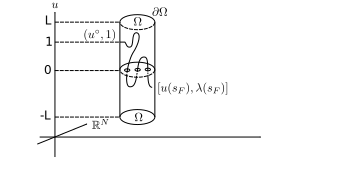
\includegraphics{vol79-fig/fig79-23.eps}
\smallskip
\caption{}
\label{chap3-fig3.5} 
\end{figure}

\begin{proof}
In $\mathbb{R}^{N+1}$, we consider the cylinder $K \equiv \bar{\Omega}
\times [-L, L]$, where $L$ is defined as in
\eqref{chap3-sec3.24-eq3.24d}. See 
Fig.~\ref{chap3-fig3.5}. Then for any fixed $u^0 \in \partial \Omega$, we have
$G(u, \lambda) \neq 0$ on the bases of $K: \lambda = \pm L$ and $u \in
\bar{\Omega}$. But on the cylindrical surface of $K$ there is at least one
solution of \eqref{chap3-sec3.24-eq3.24a}, Viz. at $(u, \lambda ) =
(u^0,1)$. Now 0 is a regular value and  
$$
\frac{\partial
G(u,\lambda)}{\partial(u,\lambda)}|_{(u^0,1)}=[F'(u^0),-F(u^0)]. 
$$  

By assumption (\ref{chap3-sec3.22-eq3.22}a), $F'(u^0)$ is
nonsingular. Hence there is a 
$C^1$ arc $\Gamma (s)\equiv [u(s),\lambda (s)]$ which satisfies
(\ref{chap3-sec3.24-eq3.24a},b,d). 
Taking $s$ as the arclength,\pageoriginale we obtain
(\ref{chap3-sec3.24-eq3.24}c) 
also. Choose the sign of $(\dot{u} (0), \dot{\lambda} (0))$ so that $\Gamma
(s) \in K$ for $s > 0$; that is $\dot{u} (0)$ at $u^0$ points into
$\Omega$. Continuity along $\Gamma (s)$ determines the orientation of
the tangent $(\dot{u}(s),\dot{\lambda} (s))$ satisfying
(\ref{chap3-sec3.24-eq3.24}c) in 
the interior of $K$. Since $L$ is so large that $G$ does not vanish
for $| \lambda| = L$, the path $\Gamma (s)$ for $s > 0$ cannot meet
the bases of $K$. The path $\Gamma (s)$ cannot terminate in the
interior since if it had an interior point must lie on $\Gamma$. Then
the implicit function theorem gives a contradiction, since 0 is a
regular value. Thus $\Gamma(s)$ must meet the cylindrical surface of
$K$ for some $s = s_F > 0$. Since the tangent $(\dot{u}
(s_F),\dot{\lambda} (s_F))$ to $\Gamma(s)$  at $s_F$ cannot point into
$K$, it follows that $\dot{u}(s_F)$ cannot point into $\Omega$ at
$u(s_F) \in \partial \Omega$. 
   
Multiplying (\ref{chap3-sec3.24}b) by $\lambda (s)$ and using
\eqref{chap3-sec3.24-eq3.24a}: 
$$
\lambda (s). F'(u) \dot{u}(s) - \dot{\lambda} (s) F (u(s) = 0 \text{
  on } \Gamma . 
$$
$F'(u)$ is nonsingular at $u = u^0$ and $u = u(s_F)$. Therefore at
points, we have: 
$$
\lambda (s)\dot{u}(s) = \dot{\lambda}(s) (F'(u(s)))^{-1} F(u(s)) 
$$

Note that $\dot{\lambda} (0)$ and $\dot{\lambda} (s_F)$ are not zero,
since $F'(u(s))$ is nonsingular for $s = 0$ and $s_F$. Now using the
boundary condition (\ref{chap3-sec3.22-eq3.22}b), We can deduce that 
\begin{equation*}
\frac{\lambda (0)}{\dot{\lambda} (0)} \frac{\lambda
  (s_F)}{\dot{\lambda}(s_F)} < 0. \tag{3.25}\label{chap3-sec3.24-eq3.25}  
\end{equation*}

Both $\lambda (0) \dfrac{\dot{u}(0)}{\dot{\lambda}(0)}$ and
$\lambda(s_F) \dfrac{\dot{u}(s_F)}{\dot{\lambda}(s_F)}$ point out of
(or into) $\Omega$. But $\dot{u}(0)$ points into $\Omega$ and
$\dot{u}(s_F)$ does not, so \eqref{chap3-sec3.24-eq3.25}  follows. 

Now\pageoriginale we will show that $\dot{\lambda} (0)
\dot{\lambda}(s_F) > 0$ which 
implies $\lambda (0)\lambda (s_F) < 0$. Hence $\lambda (s_F) < 0$ and
so the theorem follows. We have:  
\begin{gather*}
G_u \cdot\dot{u} + G_\lambda  \cdot \dot{\lambda} = 0\\[3pt]
\dot{u}^T \cdot  \dot{u} +\dot{\lambda} \dot{\lambda} = 1,
\end{gather*} 
and from (\ref{chap3-sec3.11-eq3.12a},b):
$$
\dot{\lambda}(s) = \frac{\det F' (u(s))}{\det A (s)}. 
$$ 

Now $u^0$ and $u(s_F)$ are $\partial \Omega$. By assumption
(\ref{chap3-sec3.22-eq3.22}a),%raghu 
$F'(u(s))$ is nonsingular for all $u \in \partial \Omega$. Since
$\partial \Omega$ is connected, $\det F'(u(s))$ has the same sign at
$s = 0$ and $s = S_F$. Also $A(s)$ is nonsingular all along $\Gamma$,
as we had seen in the proof of theorem \ref{chap3-sec3.11}. Hence
$\dot{\lambda}(0)$ 
and $\dot{\lambda} (s_F)$ have the same sign and the proof is
complete 
\end{proof}
